
\documentclass[tikz]{standalone}
\usepackage{amsmath}
\usetikzlibrary{calc}
\definecolor{bgcol}{HTML}{171D2B}
\definecolor{acc}{HTML}{F7B538}
\definecolor{bl}{HTML}{5B8DEF}
\definecolor{rd}{HTML}{EF6461}
\begin{document}
\pagecolor{bgcol}
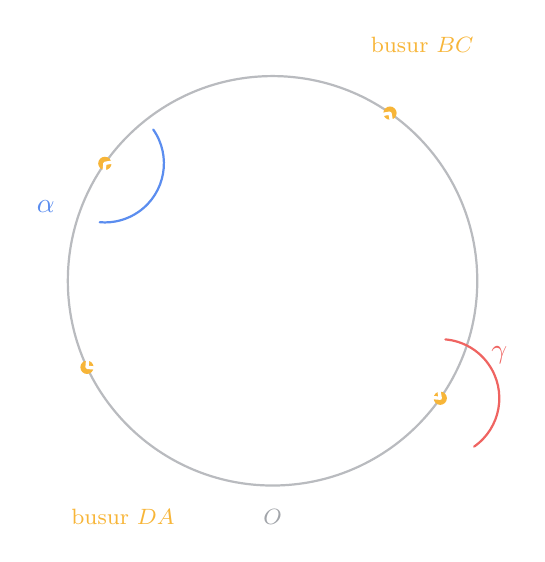
\begin{tikzpicture}[line cap=round, line join=round]
  \draw[white!70!bgcol, thick] (0,0) circle (2.6);
  \fill[white] (0,0) circle (1.6pt);
  \node[white!60!bgcol, font=\footnotesize] at (0,-3.0) {$O$};
  \coordinate (A) at (145:2.6);
  \coordinate (B) at (55:2.6);
  \coordinate (C) at (-35:2.6);
  \coordinate (D) at (205:2.6);
  \foreach \p/\dx/\dy in {A/-0.42/0.42, B/0.42/0.42, C/0.42/-0.42, D/-0.42/-0.42}
    {\fill[acc] (\p) circle (2.4pt); \node[white, font=\small] at ($(\p)+(\dx,\dy)$) {\p};}
  \draw[white, very thick] (A) -- (B) -- (C) -- (D) -- cycle;
  % interior angle alpha at A (between AB direction 35deg and AD direction ~-95deg)
  \draw[bl, thick] ([shift=(35:0.75)]A) arc[start angle=35, end angle=-95, radius=0.75];
  \node[bl] at ($(A)+(-0.75,-0.55)$) {$\alpha$};
  \draw[rd, thick] ([shift=(-55:0.75)]C) arc[start angle=-55, end angle=85, radius=0.75];
  \node[rd] at ($(C)+(0.75,0.55)$) {$\gamma$};
  \node[acc, font=\footnotesize] at (1.9,3.0) {busur $BC$};
  \node[acc, font=\footnotesize] at (-1.9,-3.0) {busur $DA$};
\end{tikzpicture}
\end{document}
